\documentclass{article}
\usepackage[margin=0.85in]{geometry}
\usepackage{graphicx,amsmath,amssymb,booktabs,listings,xcolor,placeins}
\usepackage[hidelinks,bookmarks=false]{hyperref}
\setlength{\parindent}{0pt}
\setlength{\parskip}{5pt}
\lstset{language=Python,basicstyle=\ttfamily\scriptsize,breaklines=true,
columns=fullflexible,keepspaces=true,showstringspaces=false,
frame=single,rulecolor=\color{black!20},keywordstyle=\color{blue!60!black},
commentstyle=\color{black!55}}
\title{Mobility HW1: Autonomous Driving}
\author{Cheng-Ning Huang}
\date{September 2026}
\begin{document}
\maketitle

\section{Kinematic Bicycle Model}\label{sec:vehicleControl}
\subsection{Pepy Model [1 point]}
Use a body-fixed longitudinal unit vector $\mathbf i_b=(\cos\psi,\sin\psi)$ and lateral unit vector $\mathbf j_b=(-\sin\psi,\cos\psi)$. Let $B$ be the rear-axle midpoint, $F$ the front-axle midpoint, and $G$ the center of gravity, with $BG=l_r$, $GF=l_f$, and $L=l_f+l_r$. Positive steering and yaw are counterclockwise.

\textbf{Assumptions}
\begin{enumerate}
\renewcommand{\labelenumi}{(\arabic{enumi})}
\item The rigid vehicle moves on a flat plane, i.e., roll, pitch, and changes in wheelbase are neglected.
\item The two front wheels and the two rear wheels are each replaced by one equivalent wheel.
\item Each wheel rolls along its own orientation with zero lateral tire slip; rear steering is zero.
\item In the Pepy equations, $(X,Y)$ and speed $V$ refer to the rear-axle midpoint. Steering satisfies $|\delta_f|<\pi/2$.
\end{enumerate}

Rear-wheel rolling implies $\mathbf v_B=V\mathbf i_b$. For a rigid body with yaw rate $r=\dot\psi$,
\[
\mathbf v_F=\mathbf v_B+r\mathbf k\times L\mathbf i_b
           =V\mathbf i_b+Lr\mathbf j_b.
\]
The front wheel has a lateral normal $-\sin\delta_f\mathbf i_b+\cos\delta_f\mathbf j_b$. Zero velocity along that normal gives
\[
-V\sin\delta_f+Lr\cos\delta_f=0
\quad\Rightarrow\quad r=\frac{V}{L}\tan\delta_f.
\]
The rear-axle global velocity components now give
\[
\boxed{\dot X=V\cos\psi,\qquad \dot Y=V\sin\psi,\qquad
\dot\psi=\frac{V}{l_f+l_r}\tan\delta_f.}
\]
This derivation uses geometry and rolling constraints, without force or inertia equations.

\subsection{Kong Model [1 point]}
Retain the physical assumptions above, but define $(X,Y)$ and speed $V$ at the center of gravity $G$, and denote the rear-axle speed by $V_B$. Since $G=B+l_r\mathbf i_b$,
\[
\mathbf v_G=V_B\mathbf i_b+l_rr\mathbf j_b
=V\cos\beta\mathbf i_b+V\sin\beta\mathbf j_b.
\]
Therefore $V_B=V\cos\beta$ and $l_rr=V\sin\beta$. Combining these with $r=V_B\tan\delta_f/L$ yields
\[
\tan\beta=\frac{l_rr}{V_B}=\frac{l_r}{L}\tan\delta_f,
\qquad \beta=\arctan\left(\frac{l_r}{L}\tan\delta_f\right).
\]
Rotating the center-of-gravity velocity into the global frame gives
\[
\boxed{\dot X=V\cos(\psi+\beta),\qquad
\dot Y=V\sin(\psi+\beta),\qquad
\dot\psi=\frac{V}{l_r}\sin\beta.}
\]

\subsection{Discussion [2 points]}
\subsubsection{Vehicle Slip Angle - Pepy}
The absence of $\beta$ in the Pepy equations is a consequence of choosing the rear axle as the reference point. With an unsteered rear wheel and ideal rolling, its velocity aligns with the body. The center of gravity still has lateral velocity $l_r\dot\psi$, so its vehicle sideslip angle is
\[
\boxed{\beta=\arctan\left(\frac{l_r}{l_f+l_r}\tan\delta_f\right).}
\]
Thus the center-of-gravity sideslip is generally nonzero while turning, despite zero tire slip.

\subsubsection{Vehicle vs. Tire Slip}
Vehicle sideslip compares the body axis with the center-of-gravity velocity:
\[\beta=\operatorname{atan2}(v_y,v_x).\] Tire slip angle compares a wheel's orientation with its local velocity direction. Following Lecture 4, p. 44~\cite{modeling}, use wheel direction minus velocity direction:
\[
\alpha_f=\delta_f-\arctan\frac{v_y+l_fr}{v_x},\qquad
\alpha_r=-\arctan\frac{v_y-l_rr}{v_x}.
\]
The quantities are related through the vehicle velocities, but need not vanish together. In an ideal kinematic turn, both tire slip angles vanish while $\beta$ is nonzero. Conversely, with $v_y=0$ but nonzero yaw rate or steering, $\beta=0$ while tire slip can be nonzero. In the small-slip dynamic model, the associated lateral axle forces are $F_{yf}=2C_f\alpha_f$ and $F_{yr}=2C_r\alpha_r$.

\subsection{Implementation [3 points]}
I implement the Pepy equations independently using fourth-order Runge--Kutta, starting from $(0,0,0)$ with $l_f=l_r=1.5$ m. Speed is constant in each run and the nominal time step is $0.01$ s. Square-wave switches lie on integration boundaries, i.e., the final RK4 stage uses the left limit at each switch.

\subsubsection{$\delta$ equals a nonzero constant}
At $V=5$ m/s, $\delta_f=0.10,0.25,0.45$ rad produces circles with signed radius $R=L/\tan\delta_f$ and curvature $\kappa=\tan\delta_f/L$, so larger positive steering produces a smaller circle. Each simulation lasts $40$ s, completing even the largest circle, and agrees with the analytic solution $X=R\sin(Vt/R)$, $Y=R[1-\cos(Vt/R)]$, $\psi=Vt/R$ within $10^{-7}$ in the state components.
\begin{figure}[htbp]\centering
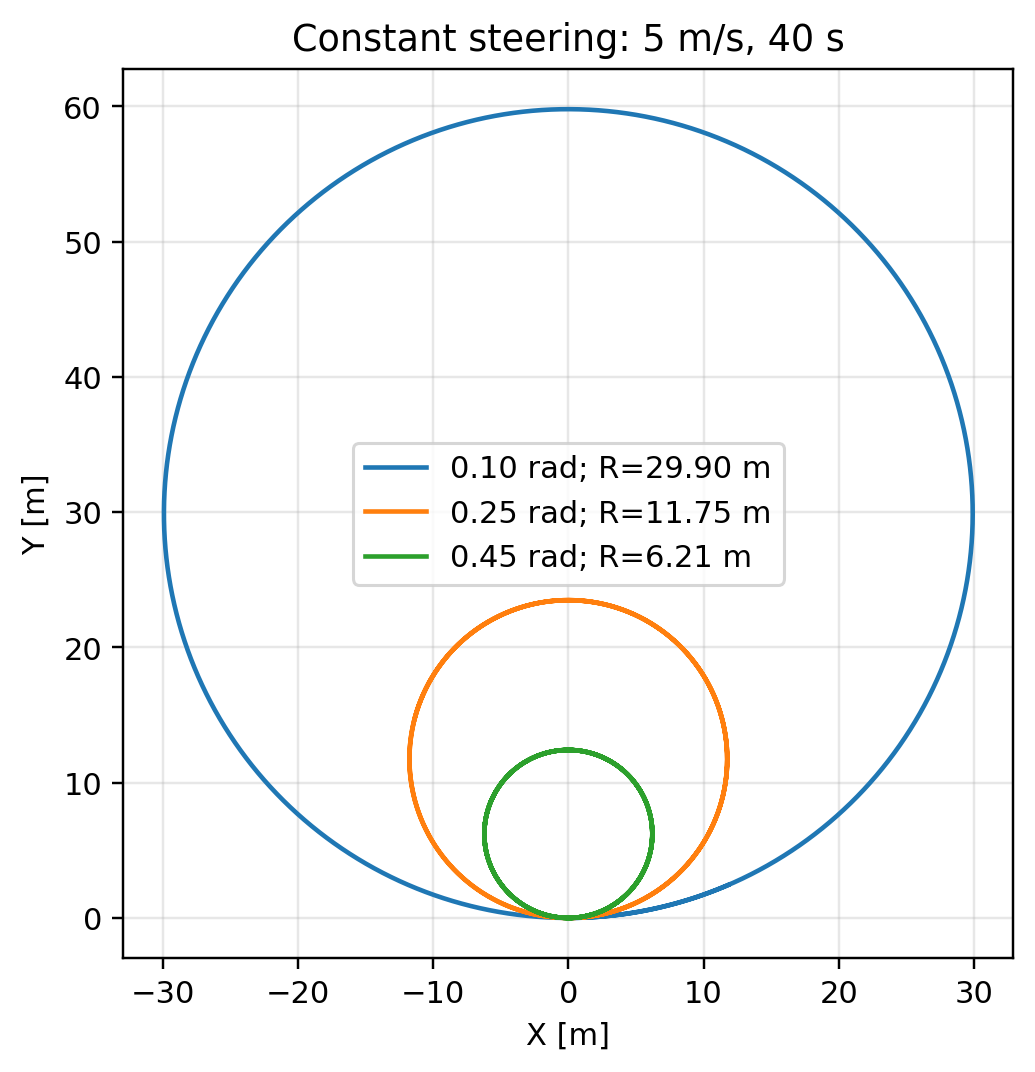
\includegraphics[width=.72\linewidth]{figures/constant.png}
\caption{Constant steering trajectories on equal scales.}
\end{figure}\FloatBarrier

\subsubsection{$\delta$ equals $\sin(t)$}
Before simulation, I predicted alternating curvature with a net lateral displacement because, for small $a$ in $\delta_f=a\sin t$, $\psi(t)\approx Va(1-\cos t)/L$. The simulated trajectories agree with this prediction. Comparing $V=2,5$ m/s and $a=0.2,0.6$ rad over two periods shows that larger steering amplitudes increase peak curvature and departure from the small-angle approximation, while higher speeds increase traveled distance and yaw excursion per input period.
\begin{figure}[htbp]\centering
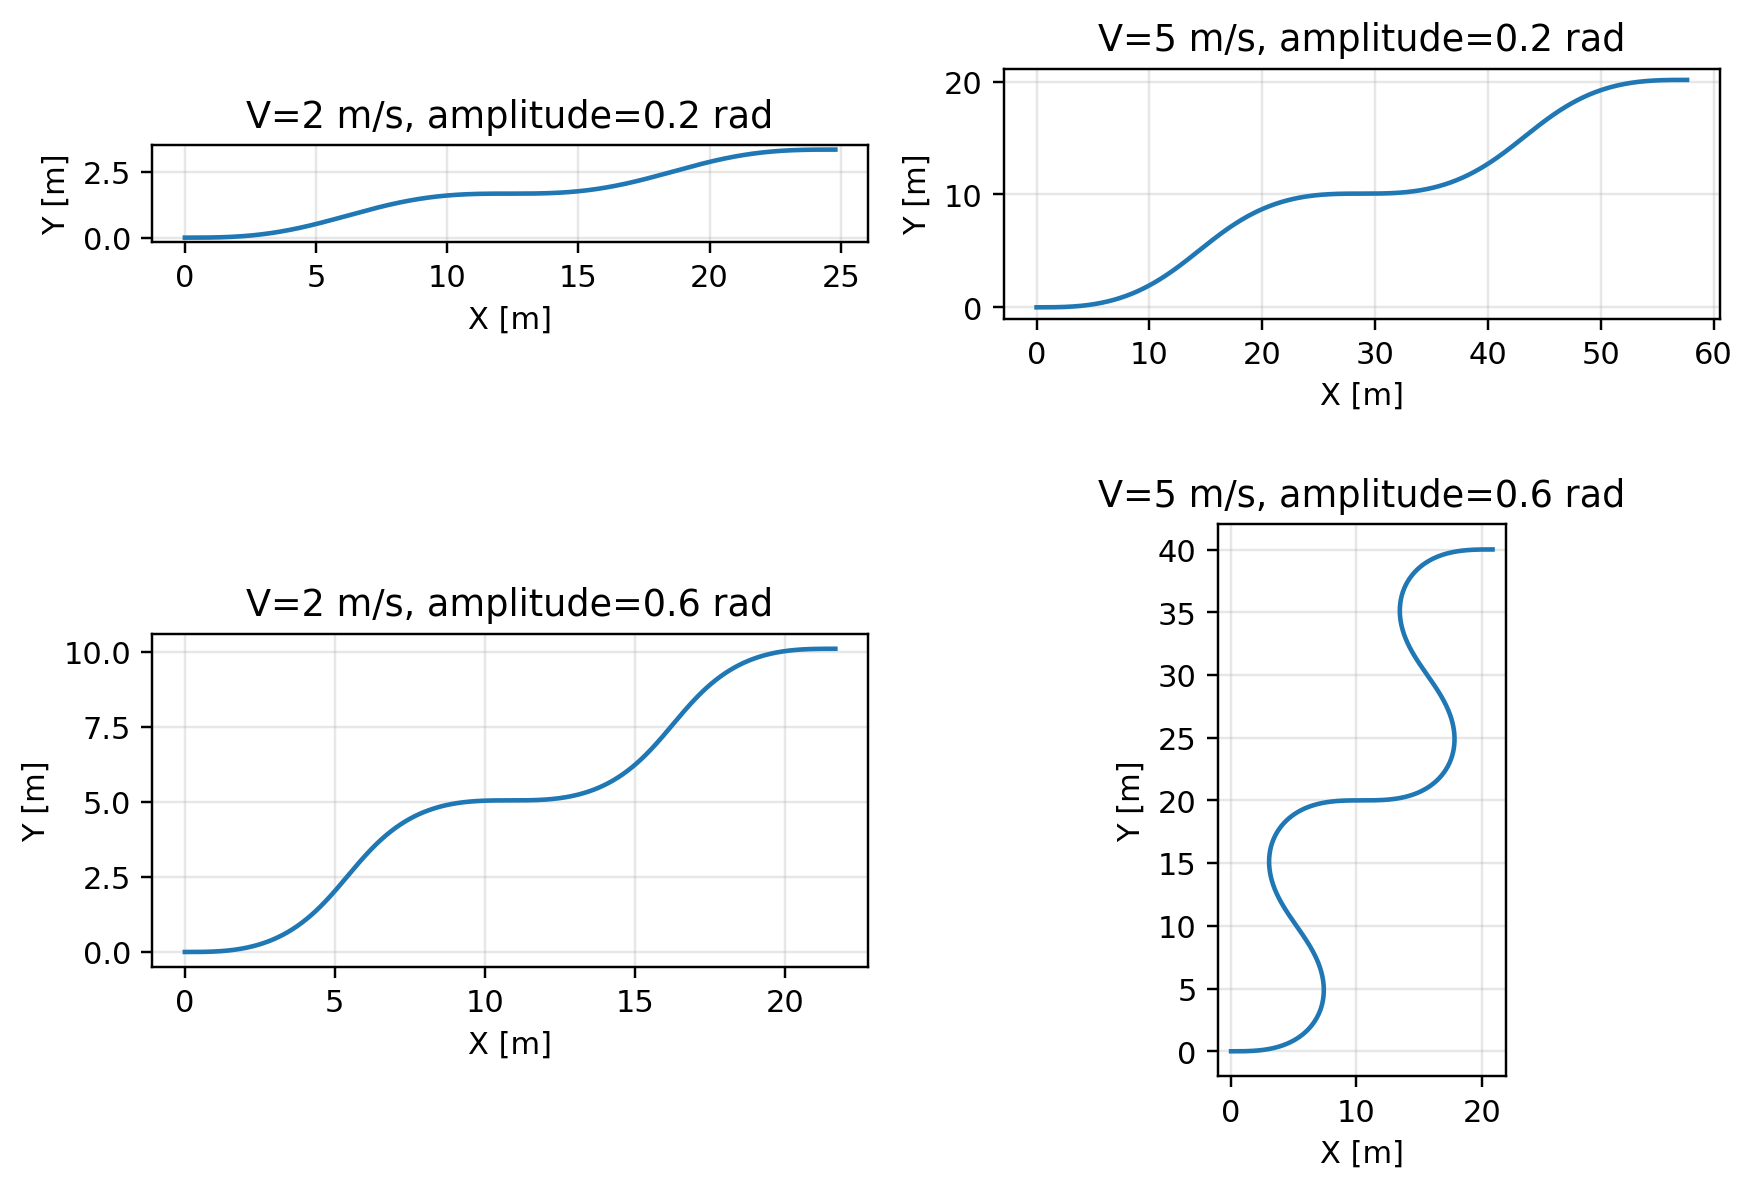
\includegraphics[width=.87\linewidth]{figures/sinusoidal.png}
\caption{Two speeds and two steering amplitudes; halving the RK4 step changes each terminal state by less than $10^{-6}$.}
\end{figure}\FloatBarrier

\subsubsection{$\delta$ equals a square wave}
With $V=4$ m/s and steering alternating between $\pm0.25$ rad every $2$ s, the model generates alternating circular arcs, but instantaneous steering jumps require infinite steering rate and are not physically realizable. To model an actuator, introduce an actual steering state satisfying $\dot\delta=\operatorname{clip}((\delta_{\rm cmd}-\delta)/\tau,-\dot\delta_{\max},\dot\delta_{\max})$ and use that continuous state in the vehicle equations.
\begin{figure}[htbp]\centering
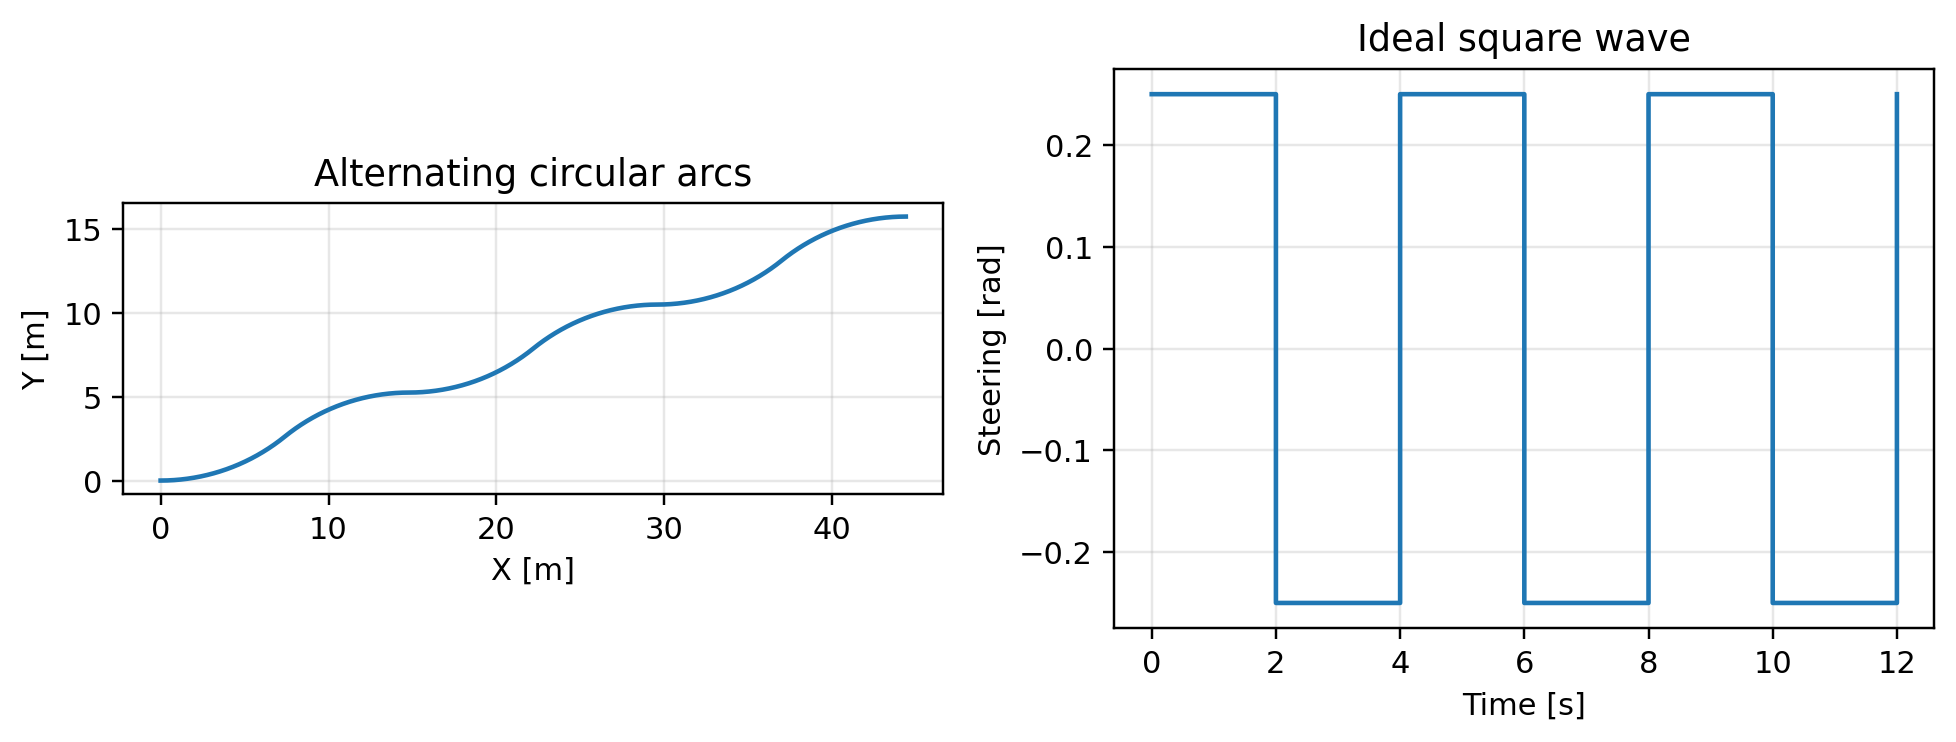
\includegraphics[width=.96\linewidth]{figures/square.png}
\caption{Ideal square-wave command and its trajectory. The actuator extension is proposed rather than included in this plot.}
\end{figure}\FloatBarrier

\section{Dynamic Bicycle Model}
\subsection{Model Set Up [0 points]}
Use the parameters specified in the assignment~\cite{assignment}: $V_x=30$ m/s, $m=1573$ kg, $I_z=2873$ kg\,m$^2$, $l_f=1.1$ m, $l_r=1.58$ m, and $C_f=C_r=80000$ N/rad. The factors of two account for the two tires per axle as in the lecture derivation.

With $x=[e_1,\dot e_1,e_2,\dot e_2]^T$, define $c=2(C_f+C_r)$, $d=2(C_fl_f-C_rl_r)$, and $h=2(C_fl_f^2+C_rl_r^2)$. Equation (10) becomes
\[
\dot x=Ax+B_1\delta+B_2\dot\psi_d,
\]
\[
A=\begin{bmatrix}
0&1&0&0\\
0&-c/(mV_x)&c/m&-d/(mV_x)\\
0&0&0&1\\
0&-d/(I_zV_x)&d/I_z&-h/(I_zV_x)
\end{bmatrix},\quad
B_1=\begin{bmatrix}0\\2C_f/m\\0\\2C_fl_f/I_z\end{bmatrix},\quad
B_2=\begin{bmatrix}0\\-d/(mV_x)-V_x\\0\\-h/(I_zV_x)\end{bmatrix}.
\]
The controllability matrix has rank four. Lecture 6, pp. 31--37~\cite{controls2}, defines $e_2=\psi-\psi_d$ and introduces $\dot e_1=v_y+V_xe_2$. Its derivation assumes slowly varying road curvature and neglects $\ddot\psi_d$. The implementation retains the supplied matrices and explicitly states the corner-input approximation below.

\subsection{Lane Change [2 points]}
The desired path is
\[
Y_d(X_d)=\begin{cases}
-5,&X_d\le5,\\
-5+(X_d-5)/18,&5<X_d<95,\\
0,&X_d\ge95.
\end{cases}
\]
Set $X_d=V_xt$, $\theta=\arctan(5/90)=0.0554985$ rad, $t_1=5/30$ s, and $t_2=95/30$ s. Initial error states are zero, corresponding to $(X,Y,\psi)=(0,-5,0)$. To avoid an undefined continuous-time derivative of the corner heading, use finite-width reference inputs with duration $\Delta t=0.01$ s and the correct signed heading change:
\[
\dot\psi_d(t)=\frac{\theta}{\Delta t}\left(
\mathbf1_{[t_1,t_1+\Delta t)}-
\mathbf1_{[t_2,t_2+\Delta t)}\right).
\]
The integrated reference heading ramps over one time step, which is an approximation to the ideal tangent at each corner. The simulation continues to $6$ s, beyond the nominal reference endpoint $(100,0)$, to measure settling. All input boundaries are handled exactly even when they fall between output samples.

\textbf{Controller design.} I searched over diagonal continuous-time LQR weights and computed the gain from the algebraic Riccati equation, following the LQR formulation in Lectures 5 and 6~\cite{controls1,controls2}. For the nominal regulation problem $\dot x=Ax+B_1\delta$, the resulting LQR gain minimizes $J=\int_0^\infty(x^TQx+\delta^2)\,dt$ with
\[
Q=\operatorname{diag}(0.1811228190,\;0.0003019885,\;5.5884459878,\;0.1870022338),\quad R=1.
\]
Solving $A^TP+PA-PB_1B_1^TP+Q=0$ and setting $K=B_1^TP$ gives
\[
\boxed{\delta=-Kx,\qquad K=[0.42558527,\;0.05773618,\;3.27261580,\;0.38541735].}
\]
The closed-loop poles are
\[
\boxed{-25.12034674,\quad-10.38059735,\quad-3.82198513\pm3.18895699i.}
\]
They all have negative real parts. No feedforward input, state reset, or steering saturation is added.

\textbf{Numerical verification.} The primary simulator uses exact matrix-exponential propagation for each constant-input interval, returning samples every $0.01$ s. A separately implemented segmented adaptive ODE integrator agrees within $1.71\times10^{-12}$ in the state components. A $0.0001$ s verification grid, including switching instants and one-second deadlines, yields:
\begin{center}
\begin{tabular}{lll}\toprule
Test in the supplied error model & Result & Required bound\\\midrule
Peak $|e_2|$ & $0.00952359$ rad & $0.01$ rad\\
First transition settling & $0.99733$ s & $1$ s\\
Second transition settling & $0.99733$ s & $1$ s\\
Peak continuous $|\dot\delta|$ & $23.80862$ rad/s & $25$ rad/s\\
Peak sampled $|\Delta\delta|/\Delta t$ & $11.64185$ rad/s & $25$ rad/s\\\bottomrule
\end{tabular}
\end{center}
Settling means both $|e_1|\le0.002$ m and $|e_2|\le0.0007$ rad hold and remain satisfied until the next transition or simulation end. The maximum transient $|e_1|$ is $0.09204$ m; no all-time lateral-error bound is specified. Steering rate is evaluated from $\dot\delta=-K[(A-B_1K)x+B_2\dot\psi_d]$, checking both one-sided derivatives at input switches as well as finite differences of the saved steering samples.
\begin{figure}[htbp]\centering
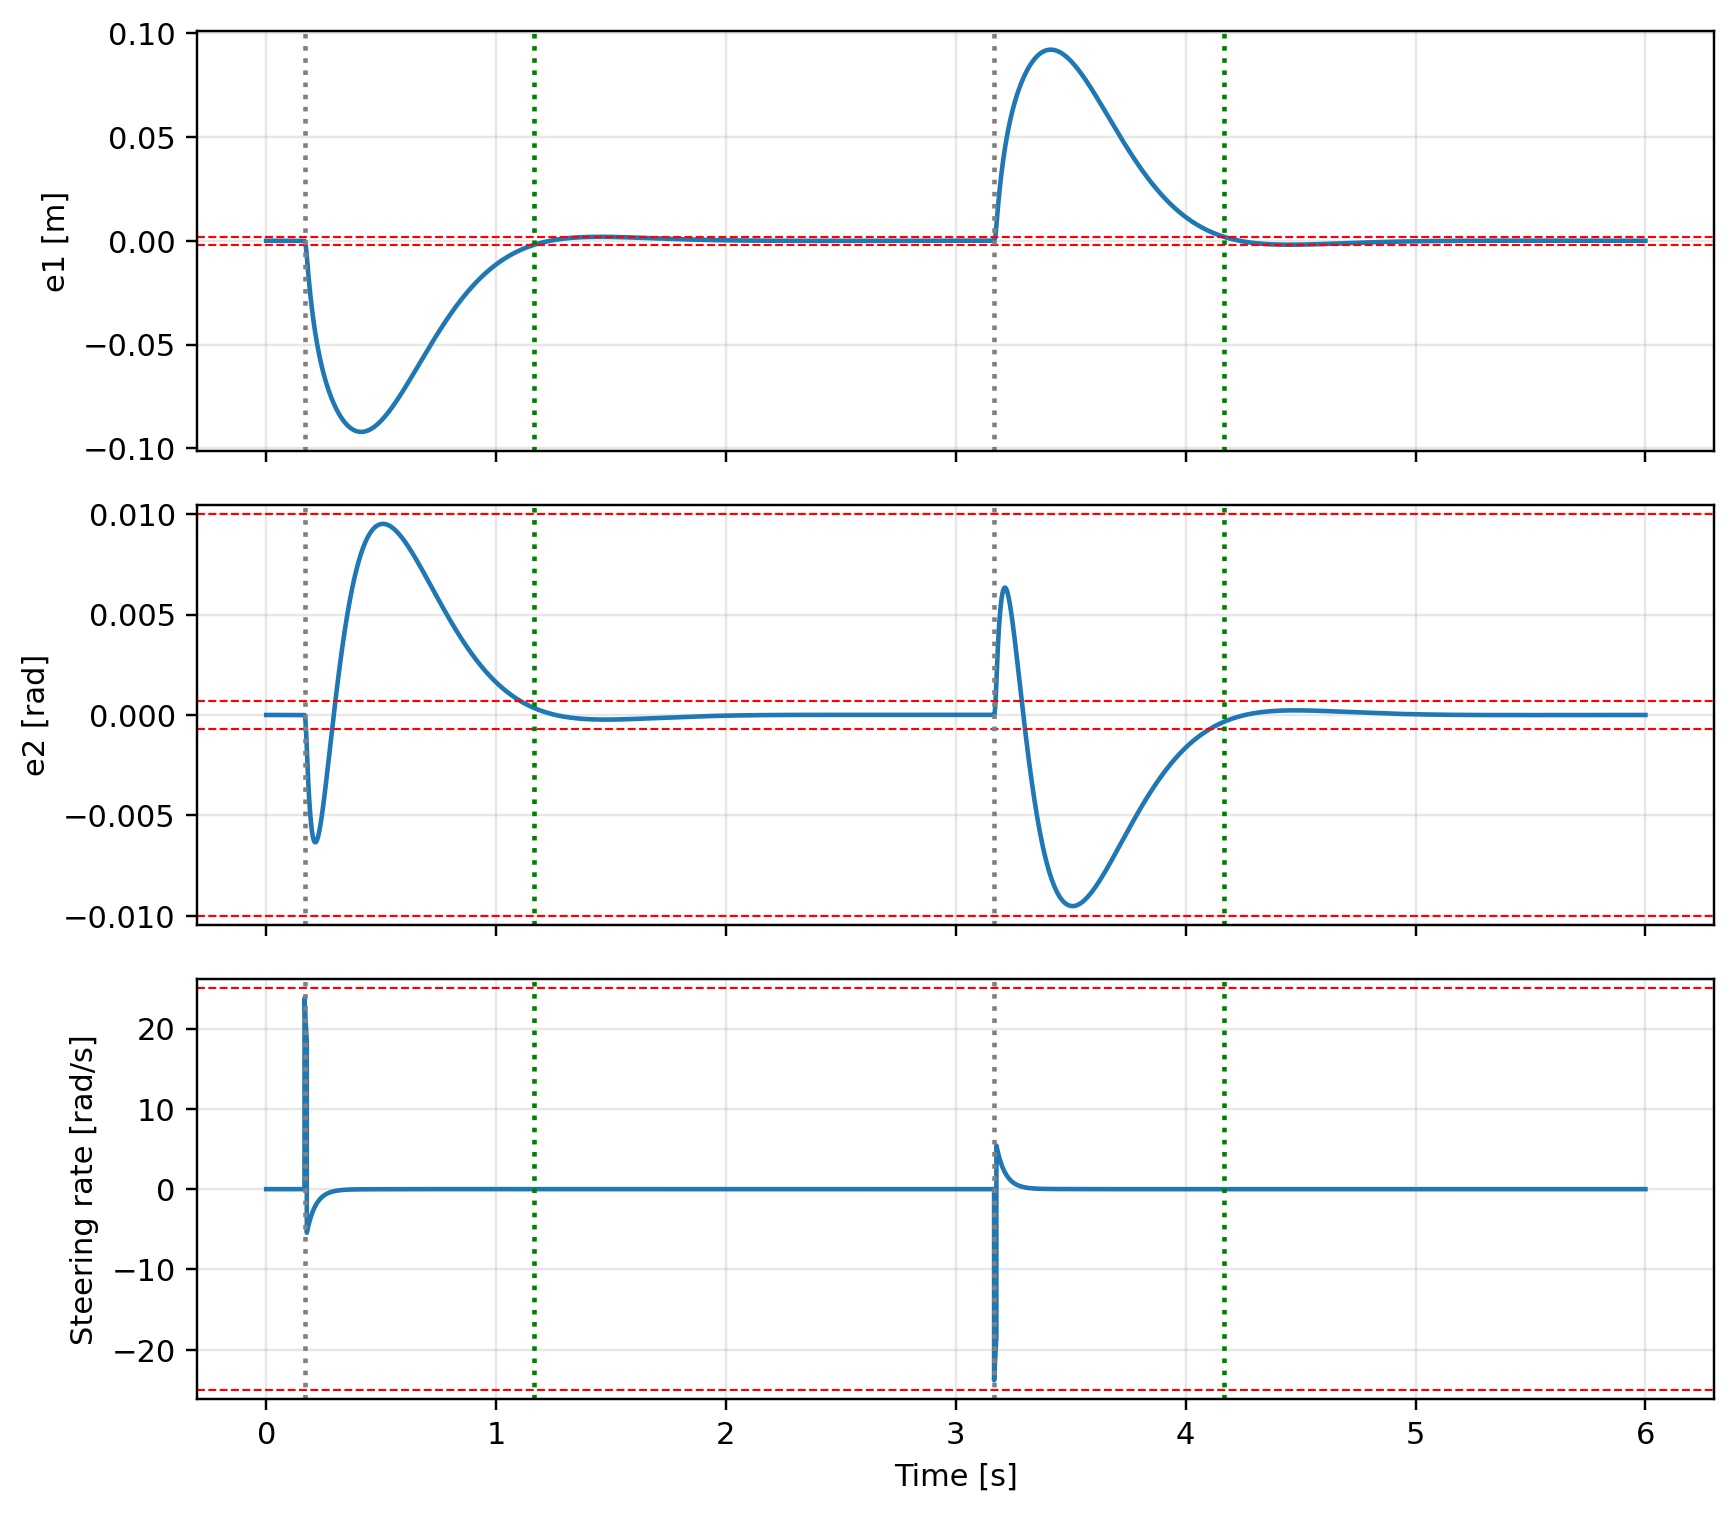
\includegraphics[width=.87\linewidth]{figures/lane_errors.png}
\caption{Course-model errors and steering rate. Gray lines mark transitions, green lines mark one-second deadlines, and red lines show the bounds.}
\end{figure}
\begin{figure}[htbp]\centering
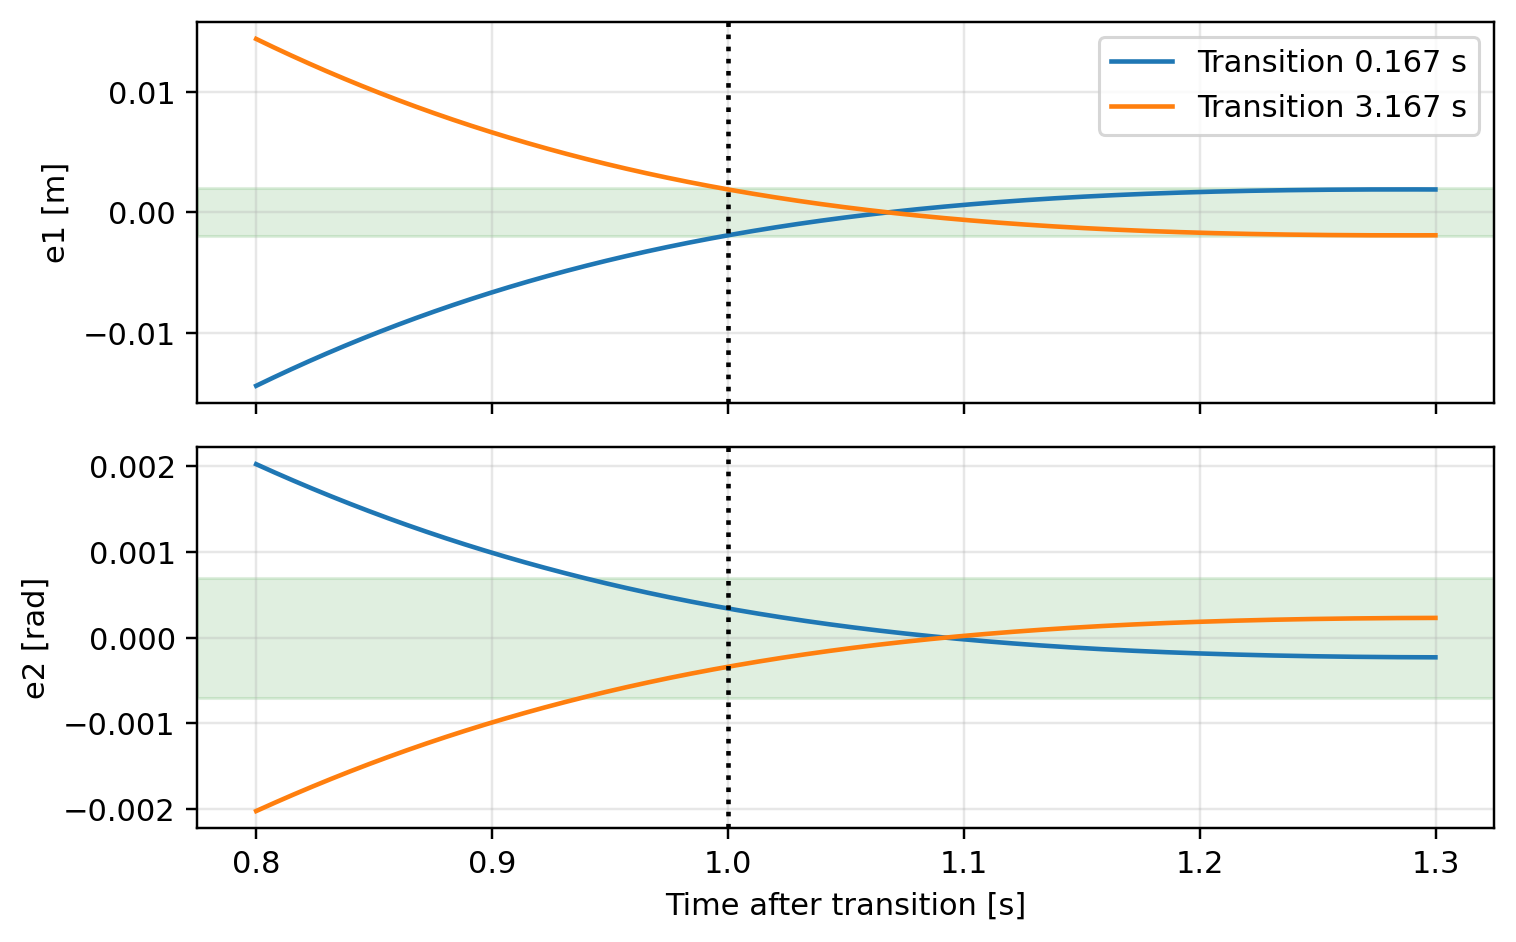
\includegraphics[width=.82\linewidth]{figures/lane_settling.png}
\caption{Both transitions aligned by elapsed time; green bands indicate simultaneous settling tolerances.}
\end{figure}\FloatBarrier

\subsection{Desired and Actual Plot [1.5 points]}
Using the body-lateral error convention illustrated in Lecture 6, p. 31~\cite{controls2}, I reconstruct the position by placing the vehicle at a displacement $e_1$ along the body-lateral axis from the selected reference point:
\[
\psi=\psi_d+e_2,\qquad
X=X_d-e_1\sin\psi,\qquad Y=Y_d+e_1\cos\psi.
\]
This reconstructs global coordinates within the course's error-model convention. Projecting the displacement back onto the body lateral axis recovers $e_1$ with maximum difference $4.52\times10^{-16}$ m. This checks the coordinate conversion, not independent physical feasibility of the corner approximation. The figures use unequal axis scales to make the small lateral deviations visible.
\begin{figure}[htbp]\centering
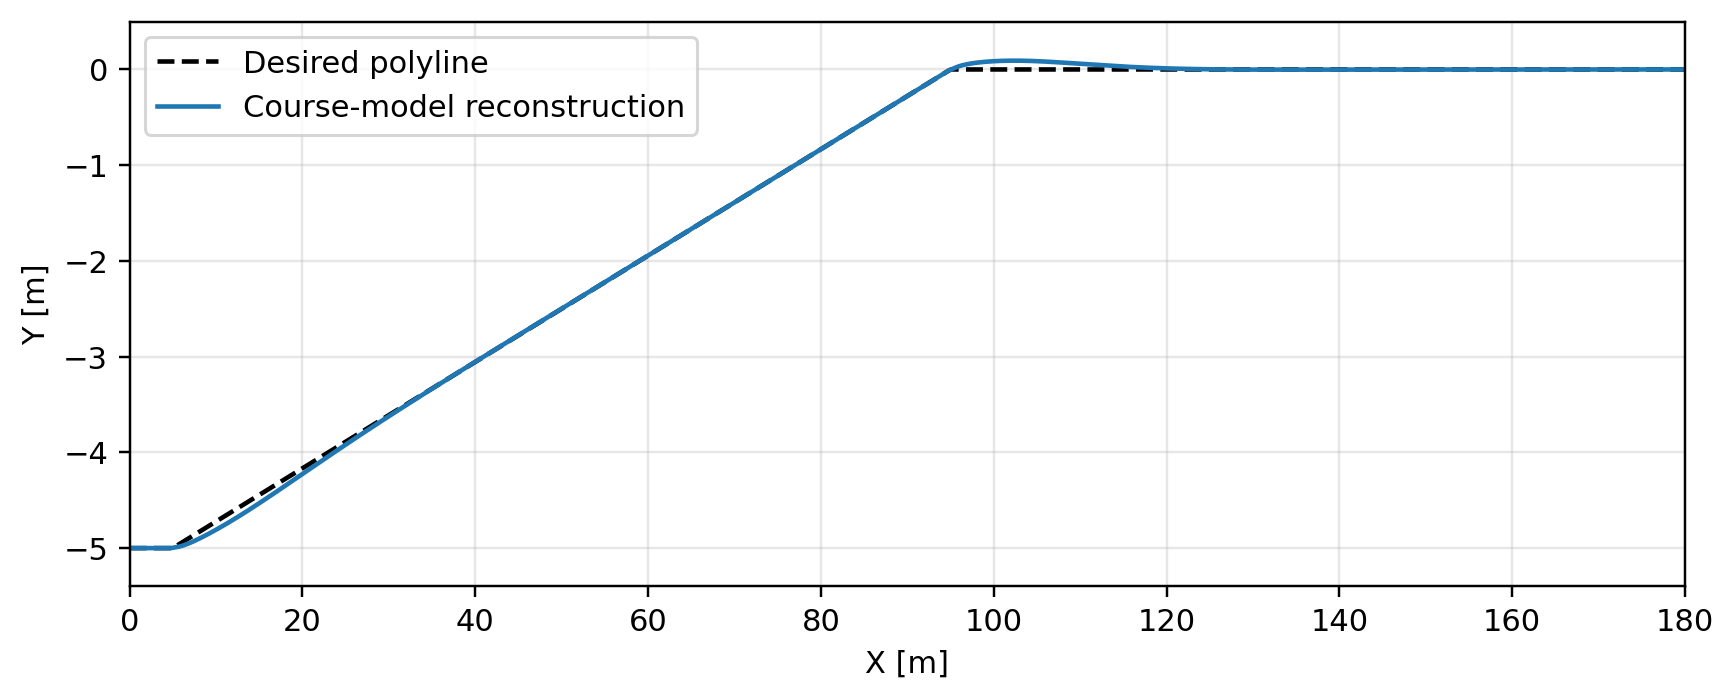
\includegraphics[width=.98\linewidth]{figures/lane_global.png}
\caption{Desired path and reconstructed global course-model trajectory.}
\end{figure}
\begin{figure}[htbp]\centering
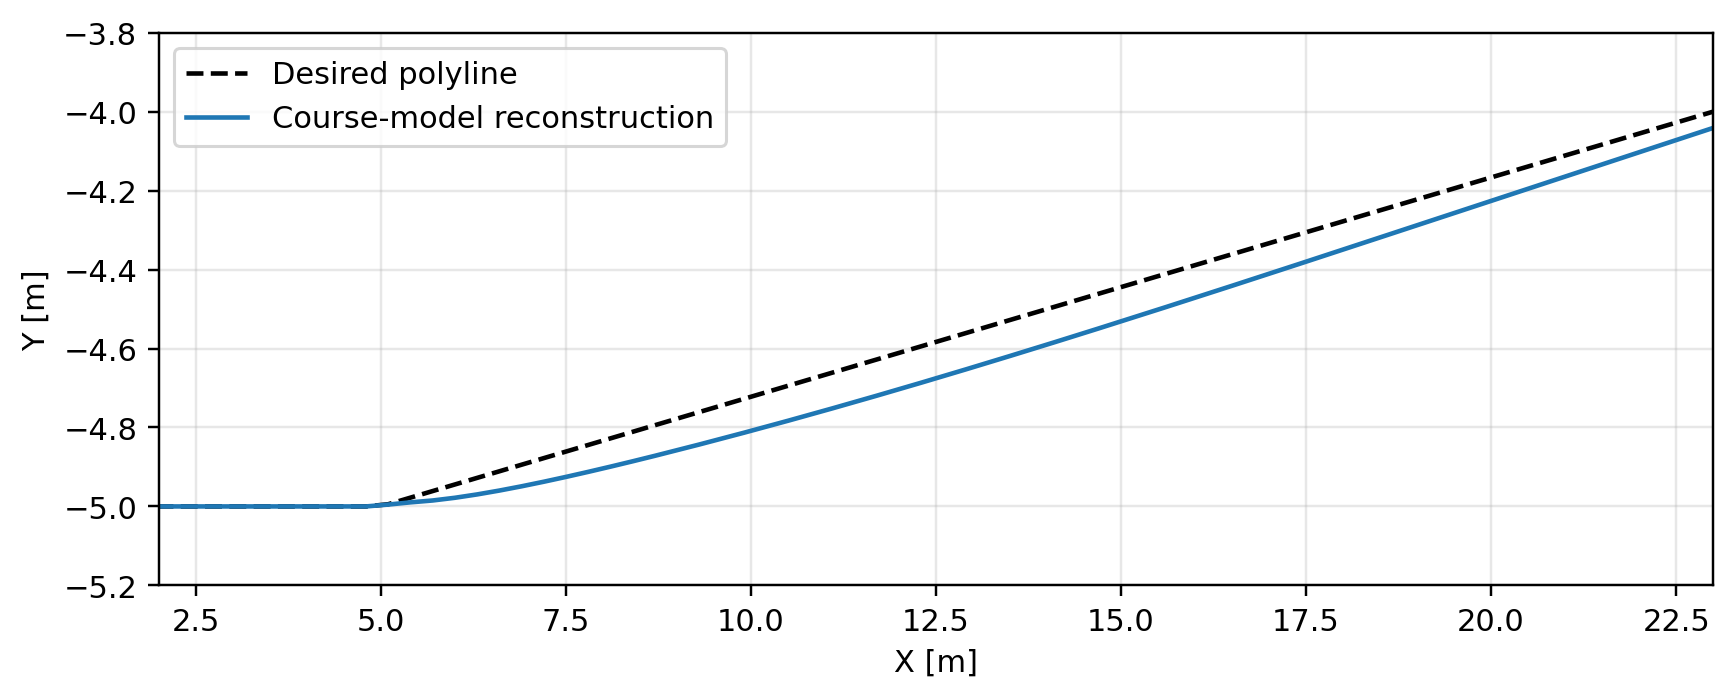
\includegraphics[width=.98\linewidth]{figures/lane_start.png}
\caption{Separate zoom at departure from the original lane.}
\end{figure}
\begin{figure}[htbp]\centering
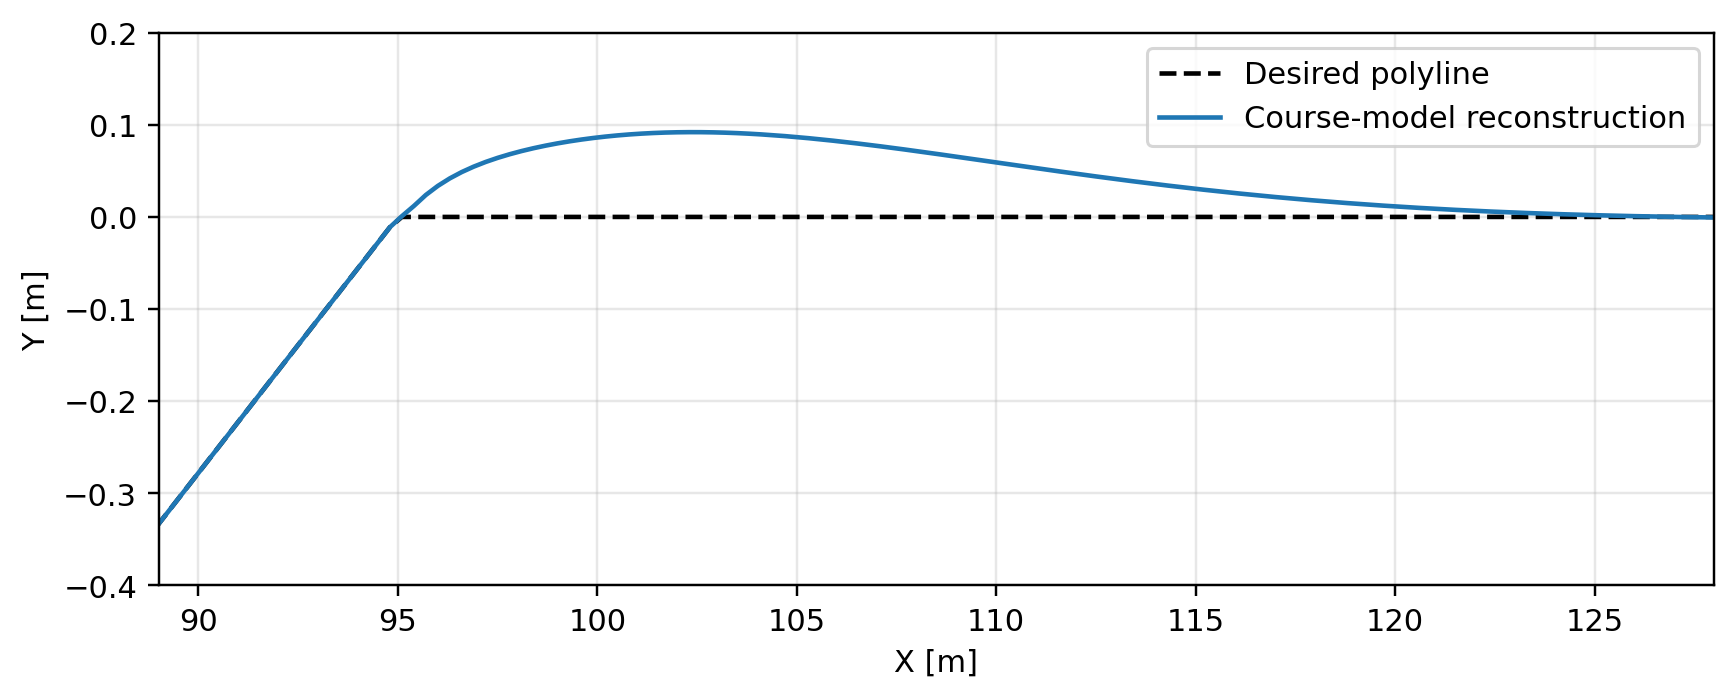
\includegraphics[width=.98\linewidth]{figures/lane_end.png}
\caption{Separate zoom at entry into the new lane.}
\end{figure}\FloatBarrier

\textbf{Endpoint and reference audit.} The error-model results above pass the stated numerical peak/rate/settling tests for the declared input representation. They do not prove every literal geometric condition. At nominal $X_d=100$ m, the reconstructed position is approximately $(100.000307,0.086239)$ m and heading is $-0.003557$ rad. Thus this candidate has not reached $(100,0)$ with zero heading there. By $6$ s the reconstructed lateral position is $4.875\times10^{-6}$ m, consistent with eventual settling.

Moreover, a finite-time reference heading ramp differs from the ideal polyline tangent. Recomputing heading error against that ideal tangent gives a peak of approximately $0.055499$ rad, rather than the smaller internal $e_2$. The script reports these as separate tests. For a continuous physical heading and an instantaneous reference jump of $\theta$, the larger of the two one-sided heading errors is at least $\theta/2=0.0277493$ rad, so the strict all-time $0.01$ rad condition cannot hold under that particular interpretation.

Consequently, this is a verified candidate for the supplied approximate error-model exercise, not a claim that the literal sharp-corner and finite-endpoint conditions are all satisfied. The provided lecture derivation does not specify a grading convention for these assignment corner transitions.
\begin{figure}[htbp]\centering
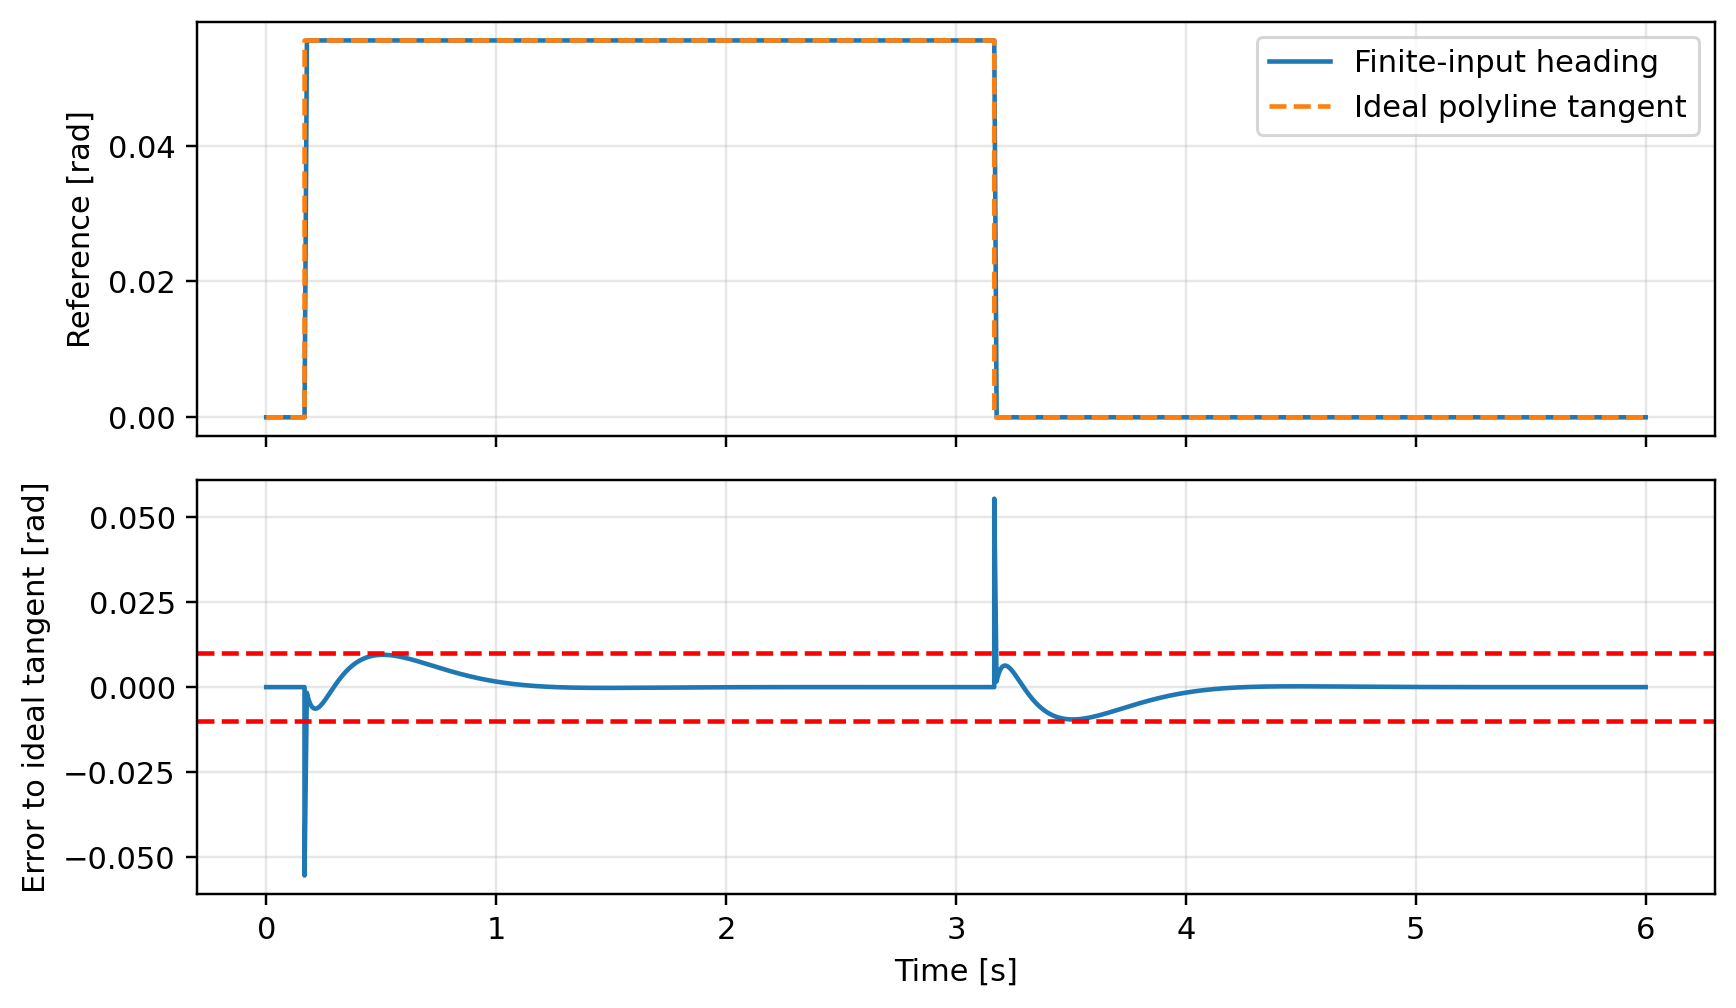
\includegraphics[width=.95\linewidth]{figures/reference_audit.png}
\caption{The finite-input heading and ideal tangent agree away from corners. The lower panel audits heading error against the ideal tangent.}
\end{figure}\FloatBarrier

\begin{thebibliography}{9}
\bibitem{assignment}
Carnegie Mellon University,
\emph{Autonomous Driving Mobility Assignment},
16-665: Robot Mobility on Air, Land, and Sea, September 2026.

\bibitem{modeling}
J. M. Dolan,
\emph{MRSD Robot Mobility: Autonomous Driving: Vehicle Modeling},
Lecture 4, Carnegie Mellon University, September 8, 2026.

\bibitem{controls1}
J. M. Dolan,
\emph{MRSD Robot Mobility: Autonomous Driving: Controls 1},
Lecture 5, Carnegie Mellon University, September 10, 2026.

\bibitem{controls2}
J. M. Dolan,
\emph{MRSD Robot Mobility: Autonomous Driving: Vehicle Control 2},
Lecture 6, Carnegie Mellon University, September 15, 2026.
\end{thebibliography}

\newpage
\section{Appendix}

\subsection{1.4.A Pepy Model constant turning implementation}
\textbf{Shared models and LQR solver: \texttt{bicycle.py}}
\lstinputlisting{bicycle.py}
\textbf{RK4, all three steering experiments, checks and plotting: \texttt{kinematics.py}}
\lstinputlisting{kinematics.py}
\subsection{1.4.B Pepy Model sinusoidal turning implementation}
The complete implementation is the \texttt{sinusoidal()} function in the preceding listing. It calls the same RK4 integrator with two step sizes for an independent refinement check.
\subsection{1.4.C Pepy Model square wave turning implementation}
The complete implementation is the \texttt{square()} function in the preceding listing. The RK4 endpoint convention treats the left and right limits of the ideal steering jumps consistently.
\subsection{2.1 Dynamic Bicycle Model Lane Change Setup}
\lstinputlisting{lane_change.py}
\textbf{Complete numerical design input: \texttt{design.json}}
\lstinputlisting[language={}]{design.json}
\end{document}